\subsubsection{xGA} 

\paragraph{Overview} 

The xGA project is focused on improving the performance, scalability,
and user productivity of the Global Arrays (GA) library for exascale
systems.  This is essential to the ECP applications that already depend
on GA such as NWChemEx\cite{xGA_NWCHEM}, GAMESS\cite{xGA_GAMESS} and
GridPACK\cite{xGA_GRIDPACK} (used as part of the Stochastic Grid
Dynamics project).  In addition, GA is being considered for use in the
ECP application QMCPACK\cite{xGA_QMCPACK}.

GA supports a shared memory-like programming model on distributed memory
platforms.  This allows users to create distributed multidimensional
arrays that can be accessed from any processor using simple one-sided
put/get/accumulate communication primitives. Data consistency is maintained
using global synchronization mechanisms that flush all outstanding communication
from the system and guarantee that arrays are in a known state.
We are extending the GA library in a number of ways to take advantage of
exascale architecture features including
deep memory hierarchies and accelerators, while continuing to tune and
improve the performance of the GA runtime.

\paragraph{Key  Challenges}

Application codes increasingly need to take advantage of emerging
hardware features to support more sophisticated scientific models. These
hardware features extend the computing model beyond the concept of one compute
thread per communication process as well as extending the memory model beyond
the idea of a single flat view of data. Some of these Exascale platform features
include massively multi-core CPUs, improved network communication speeds, the
availability of GPU accelerators, and deep memory hierarchies. Any one or more
of these capabilities promises to accelerate application codes, so long as these
features are supported by the underlying runtimes and are accessible
through easy-to-use interfaces.

Partitioned Global Address Space (PGAS) models have emerged as a popular
alternative to MPI models for designing scalable applications. These are
typically paired with a one-sided communication model and are particularly
well-suited for applications with irregular access patterns that are not easily
predicted in advance.
%At the same time, MPI remains a ubiquitous communication
%subsystem due to its standardization, high performance, and availability on leading
%platforms.
Though MPI implementations are modernizing with features such as
GPUDirect technology, PGAS models have not maintained similar advances.
Users are requesting that PGAS models provide similar, seamless
features for addressing and communicating with memory that may be located
anywhere within the memory hierarchy, including memory resident on
accelerators. They are also interested in using communication calls from
multiple independent threads within a single traditional communication process.
%Both of these present significant challenges.
The lack of a consensus model for
deep memory hierarchies makes developing a single interface for exploiting these
by GA
%, or any other application for that matter,
extremely difficult.
Supporting multi-threaded applications in a robust and efficient manner is also
likely to require significant software engineering in order to remove locks and
achieve high performance.

\paragraph{Solution Strategy}

The xGA project has three primary thrusts:
\begin{enumerate}
\item \textbf{Thread safety:} GA has not previously provided any thread safety
features or specification.
\item \textbf{Deep memory:} Users should provide hints to allocate GA
memory anywhere within the memory hierarchy, including NVMe and GPUs. 
\item \textbf{Application integration:} Any new feature should directly
benefit one or more ECP applications.
\end{enumerate}

\paragraph{Recent Progress}

\begin{enumerate}
\item \textbf{Thread safety:} GA has not previously provided any thread safety
features or specification. We have recently implemented a preliminary strategy
for thread safety that puts locks on all communication calls. In principle, this
could be fairly efficient, since communications calls are not all occurring at
the same time, but the overhead of creating and destroying the locks themselves
seems to be a severe drag on performance. We are currently reviewing individual
calls to remove global variables where possible with a view to creating
lock-free versions of these calls that can be used by a multi-threaded
application.

\item \textbf{Deep memory:} We have begun looking at developing a strategy for
creating GAs on GPU memory.

\item \textbf{Application integration:} GA is used in three applications
currently supported by ECP. These include NWChemEx (via the TAMMS runtime layer),
Stochastic Grid Optimization (via GridPACK) and GAMESS. We are also in discussions
with QMCPACK application about using GA to support large distributed lookup tables
of spline coefficients. We expect that QMCPACK, as well as potentially NWChemEx,
would benefit from a read-only property that we have been working on within GA.
We are also discussing with NWChemEx how to potentially use thread-safe calls in
GA as well as exploiting the deep memory hierarchy.

\item \textbf{Data layout:} We have developed new options for controlling the
data layout within GAs. The internal routines for accessing both local and
remote data have been completely reorganized to use an iterator model that has
eliminated a lot of redundant code in the current implementation. It has also
allowed us to implement a new 'tiled' array option guarantees that data is laid
out in user-controlled blocks that are contiguous in memory. These layouts match
layouts that are being considered by some of the linear algebra libraries and
provide options for optimizing communication by eliminating strided
communication calls. We have also begun a preliminary implementation of a
sparse data layout designed to support sparse 2D array operations. We have used
this to implement a sparse matrix-vector multiplication operation.

\item \textbf{Improved Performance:} We are continually evaluating and
improving our performance. Figure~\ref{fig:ga_bw} shows how we recently
improved the bandwidth of our strided get operation in our 5.7 release
of the Progress Rank ComEx runtime\cite{xGA_COMEX}.
\end{enumerate}

\begin{figure}[htb]
    \centering
    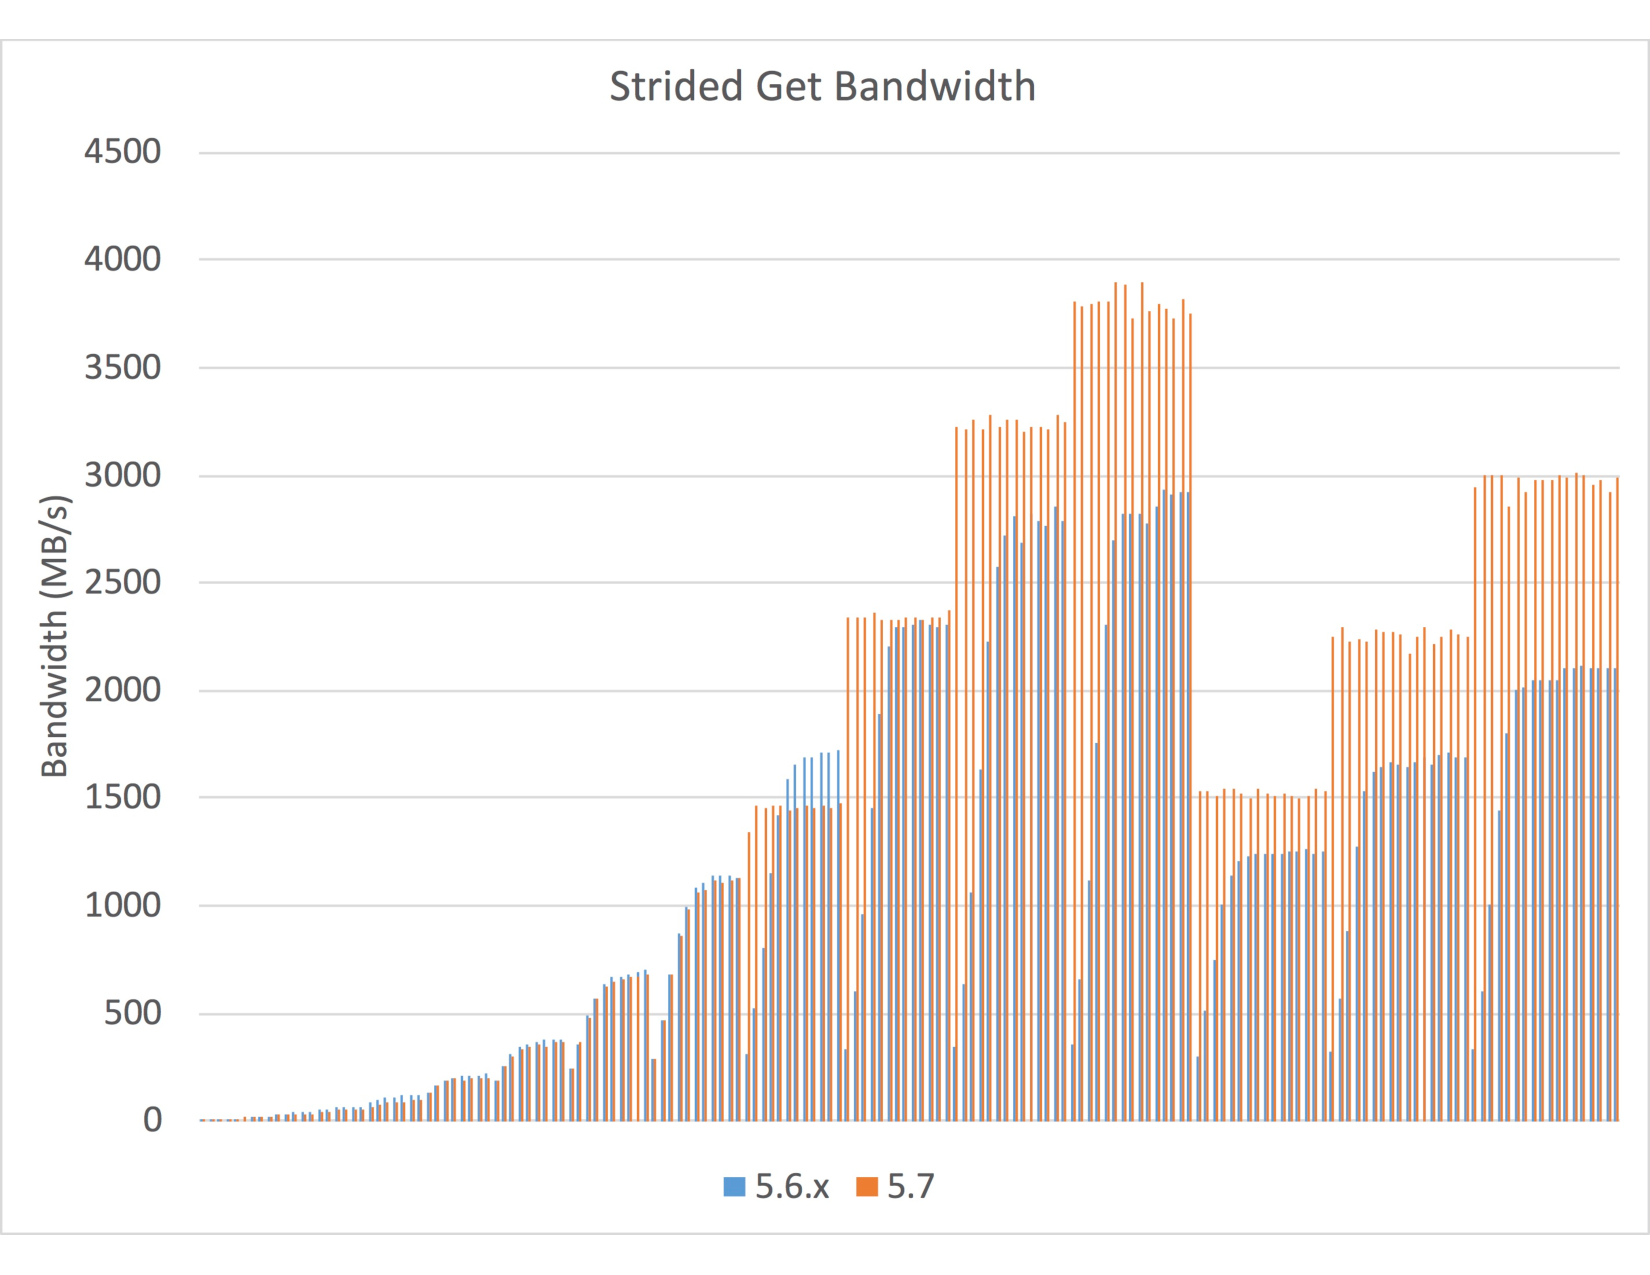
\includegraphics[width=0.7\columnwidth]{projects/2.3.1-PMR/2.3.1.05-Global-Arrays/GA_get_bw}
    \caption{\label{fig:ga_bw}Improved performance of strided get in the 5.7 release series.}
\end{figure}

\paragraph{Next Steps}

Our next steps are:

\begin{enumerate}
\item \textbf{Add hints targeting memory hierarchy allocation:} xGA will
expand its array property types allowing users to specify where memory
should be allocated. We will also continue to refine the read-only property to
include caching of requests so that we can expand the property to handle very
large arrays. Currently, the property is limited to arrays that can be stored on
a single node.
\item \textbf{Improved thread-safe performance:} We will improve our
thread-safe performance by eliminating the use of globally shared variables and
the locks that surround one-sided GA operations. In some cases, it may not be
possible to implement thread-safe solutions without locks with the existing
interface. In these cases, we will look to extending the interface to provide
thread-safe alternatives that will deliver high performance.
\end{enumerate}
